\chapter{Introduction}
\label{cha:introduction}

\dictum[Rachel Carson, \textit{Silent Spring} (1962)]{%
  The balance of nature is not a status quo; it is fluid, ever shifting, in a constant state of adjustment. \\ Man, too, is part of this balance.}%
\vskip 1em


Biology is determined by structure, patterns, and dynamics at various scales, ranging from molecular interactions to organismal behavior.
%
% Recent technologies have provided access, with an unprecedented resolution, once deemed unthinkable, into the inner workings of cells and tissues that lie on the lower-end of that scale.
%
At the lower end of that scale, single-cell genomics and transcriptomics provide now a direct window, with a resolution that was deemed unthinkable two decades ago, into the molecular makeup of individual cells, capturing vividly the inner workings of cells at any point in time.
%paving the way for a better understanding of the diversity of cell types and their functional roles. 
Similarly, advances in imaging technology provide tools to map the spatial organization of tissues and organs at the cellular and subcellular level, improving our understanding of key physiological processes.% that underlie health and disease.
%
The ability of single-cell high-throughput methods to produce routinely millions of data points holds multiple promises. They do, however,  come with an important limitation: they produce data that are not \textit{aligned}, namely, such methods are destructive assays, meaning that the same cell cannot be observed twice.
% nor fully profiled over time.
% Since many of the most pressing questions in the field involve modeling and understanding the dynamic responses of heterogeneous cell populations to various stimuli, such as environmental signals, developmental processes, genetic perturbations, or drug treatments, there is a pressing need to provide experimental and/or computational methods that can circumvent that limitation. 
This limitation is particularly acute in the field of personalized medicine, where the goal is precisely to understand the dynamic response of a patient's cells to a stimulus, and would therefore rest, in theory, on the ability to observe the same cell before and after treatment.
%
Similarly, most single-cell technologies require the physical dissection and dissociation of tissues and organs, resulting in a loss of spatial information.
%
These issues are well known challenges, and many technologies have tried to circumvent such destructive steps, notably through spatial-omics. The scalability of such methods does, however, lag behind that of single-cell sequencing, which calls for algorithmic solutions to this problem.


Our goal in this review is to highlight that the common thread in all of these problems is the recurring need to realign datasets, and that such problems can be solved using optimal transport (OT) theory \citep{villani2021topics, santambrogio2015optimal}.
OT theory, a major research area in pure mathematics in recent decades (with Fields Medals awarded to \citeauthor{villani2021topics} in 2010 and \citeauthor{figalli2017monge} in 2018), has emerged as a contender to fill in that gap \textit{in silico}. OT is best described as a toolbox that allows reconstructing how a \emph{source} population (represented as one probability distribution) can morph efficiently into another \emph{target} population, given only source and target samples. Taking for the source distribution a sample of cells pre-stimuli, and for the target, another sample of cells post-stimuli, OT can reconstruct the unobserved process and provide an informed guess to define a \emph{transport map} that relates these two cell populations. 

\begin{figure}[t]
  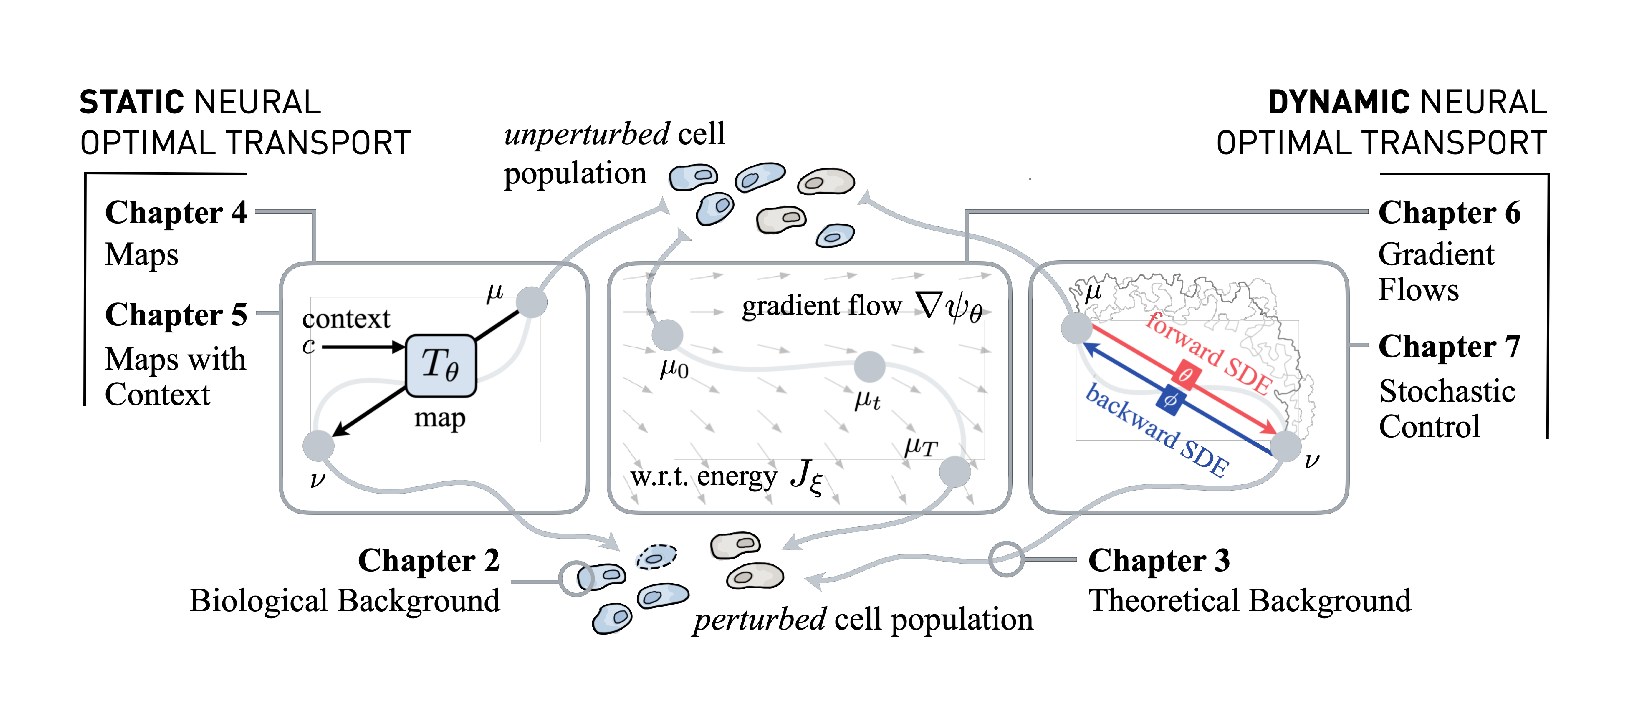
\includegraphics[width=\textwidth]{figures/fig_overview_thesis.pdf}
  \caption{Overview on ...}
\end{figure}


Applied to the analysis and modeling of single-cell biology problems, OT has been used to infer the distributions of cells' ancestors and descendants along development \citep{schiebinger2019optimal}, perform trajectory inference \citep{bunne2022proximal, forrow2021lineageot, bunne2022recovering, lavenant2021towards, schiebinger2019optimal, tong2020trajectorynet, yang2020predicting, zhang2021optimal, chizat2022trajectory}, predict perturbation responses \citep{bunne2021learning, yang2018scalable, lubeck2022neural}, integrate multi-omics data of different modalities \citep{demetci2022scot}, infer cell-cell similarity \citep{huizing2022optimal}, and integrate across scales (e.g., morphology and molecular profiling) \citep{yang2021multi}. The increasing data complexity across multiple levels of biological organization, from molecular and cellular through spatial profiling \citep{moriel2021novosparc} of tissues, and imaging of organs, cement further the status of OT as an indispensable framework for high-throughput, multimodal, and multi-scale molecular, cell, tissue, and organ biology. The effectiveness of OT comes, however, with drawbacks: because the theory builds on extremely sophisticated mathematics that blends optimization \citep{cuturi2013sinkhorn, cuturi2022optimal}, stochasticity \citep{chizat2022trajectory, bunne2022recovering} and partial differential equations \citep{bunne2022proximal}, and, more recently, deep learning \citep{tong2020trajectorynet, bunne2021learning, bunne2022supervised, yang2018scalable, lubeck2022neural, yang2021multi}, its computations are challenging even by modern ML standards.

% By leveraging the principles of optimal transport, ... and thus overcome the limitations of traditional methods and unlock new insights into the complexity of biological systems.
% ...

In this primer, we introduce the mathematical and computational principles of OT, with the goal of facilitating its use by researchers that wish to apply to novel applications. We provide the reader with intuitive explanations of how seemingly unrelated mathematical approaches for analyzing single-cell data can be unified through OT theory, and how that theory has triggered recent advances in deep learning. We provide an overview of the broad range of biological applications, demonstrating the successes of OT in the field, especially within the field of single-cell biology. With its rich properties, astonishing mathematical connections, and its innovative numerical implementations \citep{cuturi2022optimal}, OT makes for an exciting avenue of future work to make novel biological discoveries, infer personalized cancer therapies from single-cell patient samples, and push the boundaries of regenerative medicine.



